\documentclass[11pt]{article}
\usepackage[utf8]{inputenc}
\usepackage[spanish]{babel}
\usepackage[margin=2.5cm]{geometry}
\usepackage{graphicx}
\usepackage{amsmath}
\usepackage{xcolor}
\usepackage{hyperref}

\title{\textbf{Equilibrio de una carga en un sistema de cargas eléctricas}\\[4pt]
\large Informe: método de relajación y método de bisección}
\author{Sebastián Vargas Contreras}
\date{}

\begin{document}
\maketitle
\vspace{-1cm}

\section*{¿Qué se hizo?}

Hay dos cargas fijas (una en el origen, otra en $x=2$ m) y una tercera carga que se puede mover.
Además hay un ``campo extra'' no lineal que también empuja a la carga móvil. Se buscó el punto
donde todas las fuerzas se cancelan (el equilibrio), usando dos métodos distintos:

\begin{itemize}
  \item \textbf{Parte A:} un método de \emph{aproximaciones sucesivas} (relajación), que va
  corrigiendo una posición inicial paso a paso hasta que casi no cambia.
  \item \textbf{Parte B:} el método de \emph{bisección}, que busca en una línea recta el punto
  donde la energía llega a un valor determinado, partiendo el intervalo a la mitad una y otra vez.
\end{itemize}

\section*{Parte A: método de relajación}

Se partió de un punto inicial cercano a las cargas, $(x_0,y_0) = (1.0,\,0.5)$. El método corrige
la posición poco a poco:
\[
(x,y)_{\text{nuevo}} = (1-\omega)\,(x,y)_{\text{viejo}} \;+\; \omega \cdot g(x,y)_{\text{viejo}}
\]
donde $g$ es la fórmula que ``propone'' la siguiente posición, y $\omega$ (entre 0 y 1) controla
qué tan grande es cada paso: con $\omega$ chico se avanza despacio pero con más control.

\textbf{Lo que se encontró:} si se intenta dar el paso completo de una vez ($\omega=1$), el primer
salto es enorme y el método se vuelve inestable. Suavizando el avance (bajando $\omega$, o
dejando que el programa lo ajuste solo), el método sí converge, en \textbf{23 pasos}, pero termina
en un punto de equilibrio \emph{distinto} al que uno esperaría intuitivamente cerca de las cargas:
llega a $(x^*,y^*)\approx(5.95,\;6.25)$.

Esto pasa porque el punto ``obvio'' —el que está justo entre las dos cargas, sobre el eje— resulta
ser un equilibrio \emph{inestable} en la dirección perpendicular al eje: cualquier pequeño
desplazamiento hacia arriba o abajo hace que el método se aleje de él en vez de acercarse, sin
importar qué tan pequeños se hagan los pasos. En cambio, el otro punto sí es un equilibrio
\emph{estable}, y por eso es al que el método llega sin problema.

\vspace{4pt}
\noindent\textit{En otras palabras: no todo punto de equilibrio se puede alcanzar con este tipo
de método. Solo se llega a los que son ``estables'' —los que atraen— y no a los que son
``inestables'' —los que repelen apenas se aleja un poco de ellos.}

\begin{figure}[h]
  \centering
  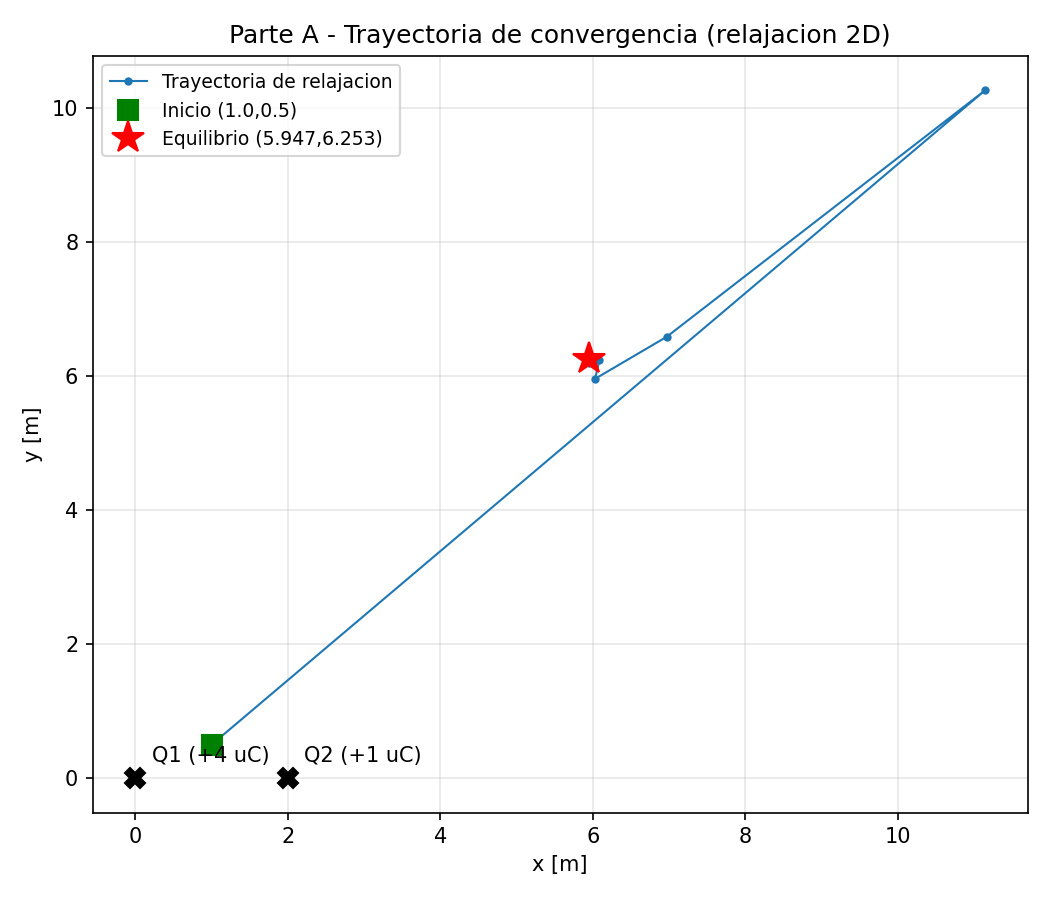
\includegraphics[width=0.68\textwidth]{parteA_trayectoria.png}
  \caption{Camino que recorre el método hasta llegar al equilibrio.}
\end{figure}

\begin{figure}[h]
  \centering
  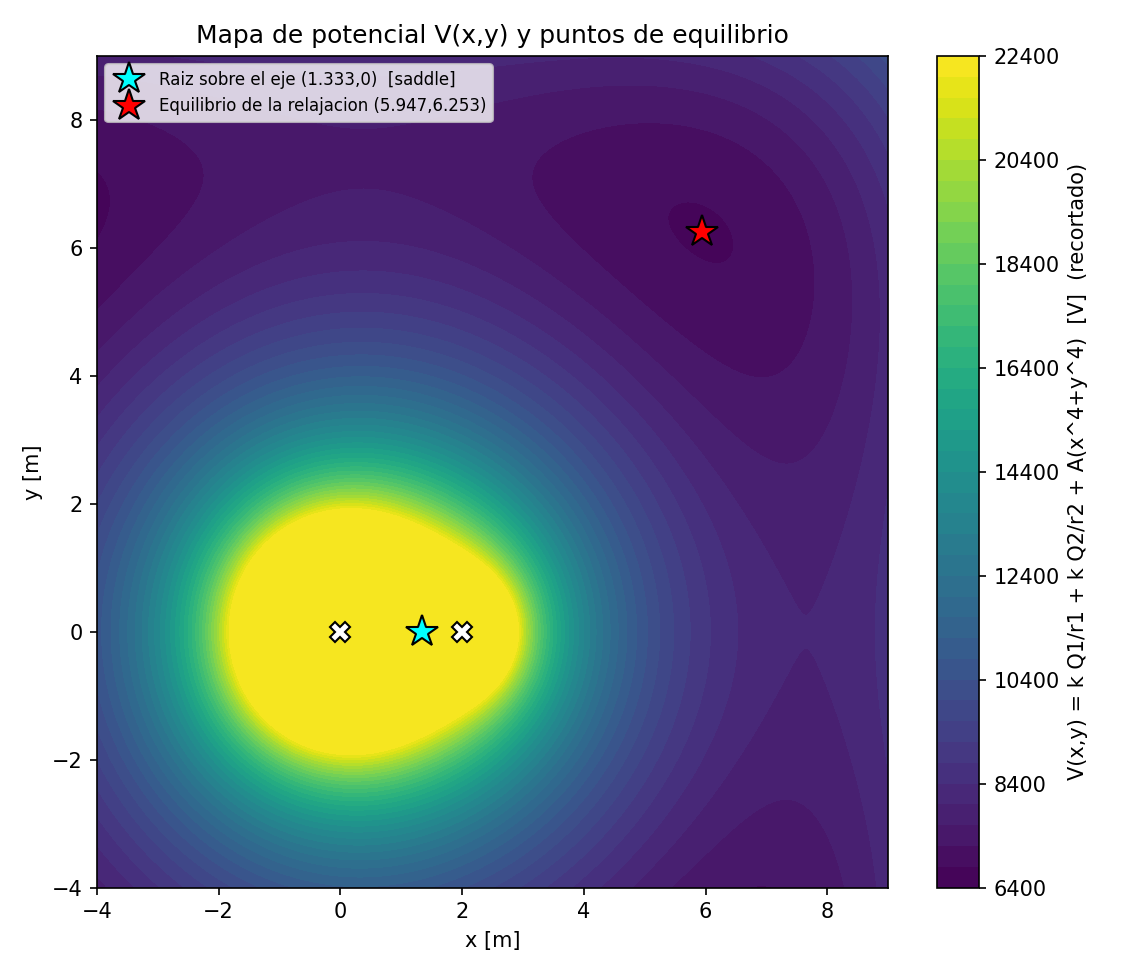
\includegraphics[width=0.72\textwidth]{mapa_potencial_equilibrios.png}
  \caption{Mapa de potencial. El punto celeste es el equilibrio inestable (sobre el eje); el
  punto rojo es el equilibrio estable al que realmente llega el método.}
\end{figure}

\clearpage
\section*{Parte B: método de bisección}

Sobre la línea que une las dos cargas, se calculó la energía $U(x)$ de la carga móvil en cada
posición, y se buscó el punto donde esa energía llega a un valor objetivo $U_0$, partiendo el
intervalo de búsqueda a la mitad en cada paso.

\textbf{Lo que se encontró:} el valor pedido originalmente, $U_0=15$ mJ, \textbf{no se puede
alcanzar} en el tramo indicado: la energía más baja posible ahí es de unos 40 mJ, así que 15 mJ
queda simplemente fuera de rango (es como buscar un punto donde la temperatura baje de 0°C en un
lugar donde nunca hace tanto frío). Para mostrar que el método sí funciona, se repitió la búsqueda
con un valor alcanzable, $U_0=45$ mJ, y ahí sí se encontraron dos soluciones: $x^*\approx0.998$ y
$x^*\approx1.601$, cada una en unas 17 iteraciones.

\begin{figure}[h]
  \centering
  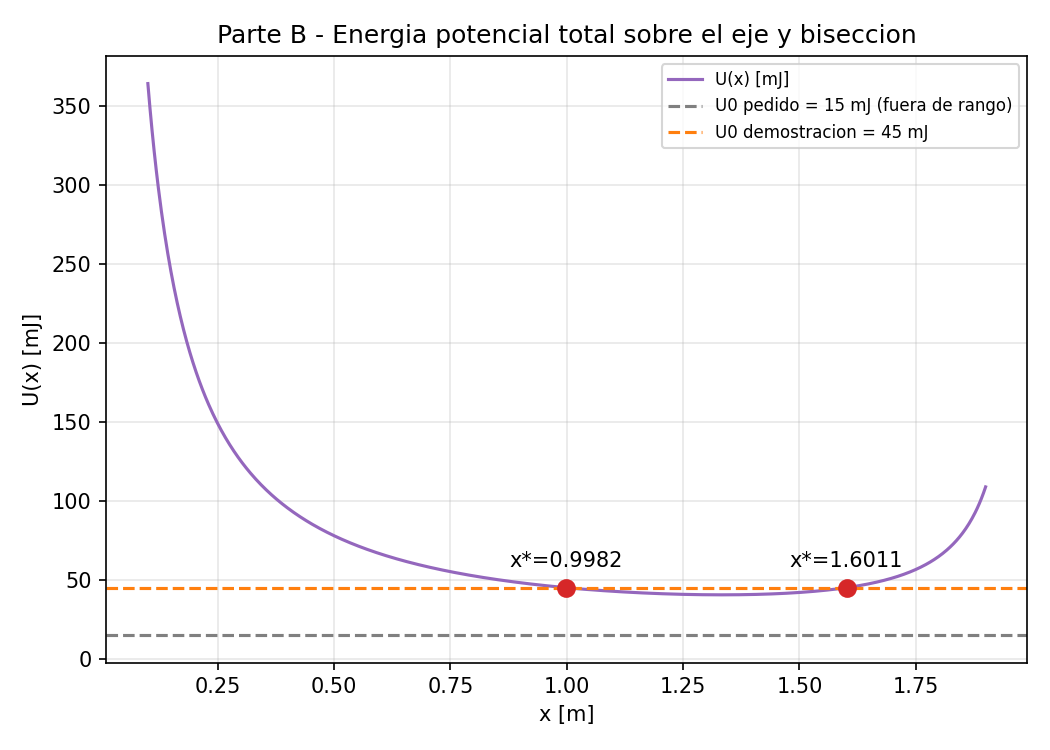
\includegraphics[width=0.68\textwidth]{parteB_biseccion.png}
  \caption{Energía a lo largo del eje. La línea gris (15 mJ) no cruza la curva; la naranja
  (45 mJ) sí, en dos puntos.}
\end{figure}

\section*{Comparando los dos métodos}

\begin{itemize}
  \item La \textbf{bisección} es muy confiable: si el valor buscado existe en el intervalo,
  siempre lo encuentra, y se puede calcular de antemano cuántos pasos va a necesitar (en este
  caso, 18 como máximo). Su único requisito es que el valor buscado realmente esté dentro del
  rango posible.
  \item La \textbf{relajación} puede ser rápida cuando funciona (aquí, 23 pasos, algo similar a
  la bisección), pero no siempre llega adonde uno espera: depende del punto de partida y de si
  el equilibrio buscado es estable o no. No hay garantía previa de que vaya a funcionar.
\end{itemize}

\begin{figure}[h]
  \centering
  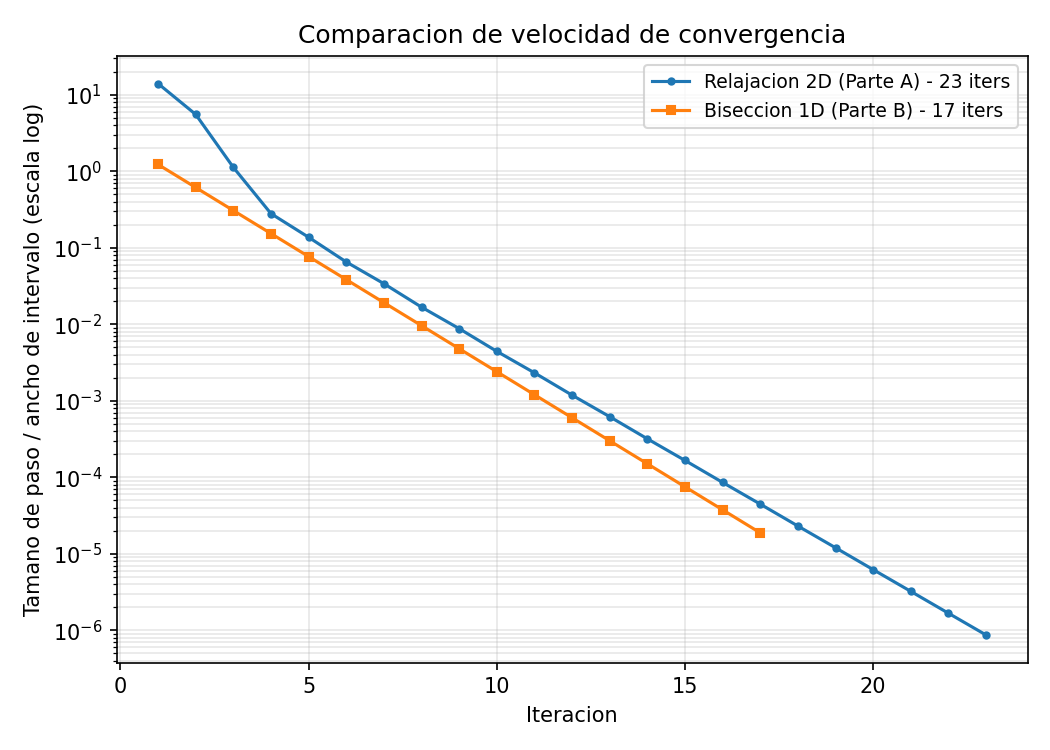
\includegraphics[width=0.68\textwidth]{comparacion_convergencia.png}
  \caption{Qué tan rápido se achica el error en cada método, paso a paso.}
\end{figure}

\end{document}
